\documentclass{article}
\usepackage{graphicx} % Required for inserting images
\usepackage{amsmath}
\usepackage{matlab-prettifier}

\title{Project Part 1: One-Dimensional Tracking Model Development}
\author{Devin Smith \\ UIN: 330000494}
\date{Applied Kalman Filtering\\AERO 689-603}

\begin{document}

\maketitle

\section{Problem Statement}

The objective of this assignment is to develop mathematical models with state variables for the one-dimensional tracking problem illustrated in Figure 1.
\begin{figure}[h]
    \centering
    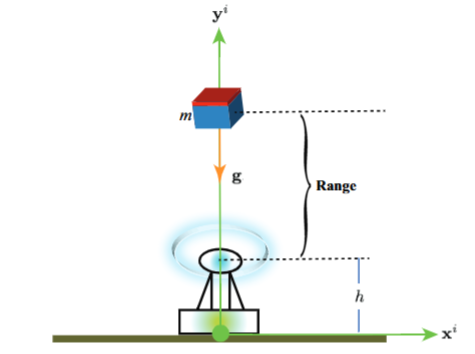
\includegraphics[width=0.75\linewidth]{Figure_1.png}
    \caption{One-Dimensional tracking problem scenario}
    \label{fig:enter-label}
\end{figure}

\subsection{Assumptions}

\begin{enumerate}
    \item Gravity, \textbf{$g$}, and height, \textit{$h$} are known constants
    \item Atmospheric drag is neglected
    \item Motion is one-dimentional (along the \textbf{$y^i$} axis)
    \item Range measurements (measured from the radar antennae dish - not the ground) are available at discrete times
\end{enumerate}

\subsection{Tasks}

\begin{enumerate}
    \item Develop mathematical models for the one-dimensional tracking problem including both continuous-time and discrete-time state-space models of the underlying dynamics and a discrete-time mathematical model of the range measurement.
    \item Clearly delineate the state variables, known inputs, and exogenous inputs (process noise and measurement noise).
    \item State all your assumptions paying special attention to your assumptions for the process noise and measurement noise.
\end{enumerate}

\section{Problem Formulation}

\subsection{Continuous-Time Model}
To properly simulate the mathematical model, an understanding of the continous-time dynamics of the falling object is needed.

\subsubsection{Dynamics}
A vector $\underline{r}$ can be defined as the position of the falling object as seen from the ground (not to be confused with the range). Furthermore, a vector $\underline{v}$ is then defined as the velocity of the falling object, and a vector $\underline{g}$ is defined as the applied gravitational acceleration. With these variables, Equations 1 and 2 can be derived (assuming we know the dynamics perfectly).

\begin{equation}
    \underline{\dot{r}}(t) = \underline{v}(t)
\end{equation}
\begin{equation}
    \underline{\ddot{r}}(t) = \underline{\dot{v}}(t) = -\underline{g}
\end{equation}

 These linear equations of motion can be rearranged as a state-space model described in Equation 3, where $\underline{x}$ is a state vector, $\underline{u}$ is a control vector, and a process noise vector $\underline{w}$ is introduced. The matrices $\mathbf{F}$ and $\mathbf{G}$ contain the dynamics of the equations of motion.

\begin{equation}
    \underline{\dot{x}}(t) = \mathbf{F}(t)\underline{x}(t) + \mathbf{G}(t)\underline{u}(t) + \underline{w}(t)
\end{equation}

In future iterations of this problem, motion will not be assumed to be one-directional, therefore, the state-space model is derived with compatibility for two-dimensional motion. The state vector is defined to contain position and velocity for both the \textbf{$x^i$} and \textbf{$y^i$} axes, and the control vector must be defined as the applied gravitational acceleration. For one-dimensional motion, the process noise can be defined as an acceleration applied along the \textbf{$y^i$} axis. Plugging in these definitions into Equation 3 gives the following, where $\underline{\dot{x}}$, $\underline{x}$, $\underline{u}$, $\underline{w}$, $\mathbf{F}$, and $\mathbf{G}$ are defined.

\begin{equation*}
    \begin{bmatrix} \dot{r_x}(t) \\ \dot{r_y}(t) \\ \dot{v_x}(t) \\ \dot{v_y}(t) \end{bmatrix} = 
    \begin{bmatrix} 0 & 0 & 1 & 0 \\ 0 & 0 & 0 & 1 \\ 0 & 0 & 0 & 0 \\ 0 & 0 & 0 & 0 \end{bmatrix}
    \begin{bmatrix} r_x(t)\\r_y(t)\\v_x(t)\\v_y(t) \end{bmatrix} +
    \begin{bmatrix} 0 & 0 \\ 0 & 0 \\ 0 & 0 \\ 0 & 1 \end{bmatrix}
    \begin{bmatrix} 0\\-g \end{bmatrix} +
    \begin{bmatrix}
        0 \\ 0 \\ 0 \\ w(t)
    \end{bmatrix}
\end{equation*}

Process noise $\underline{w}$ is defined as white noise, with characteristics shown below. $\mathbf{Q}_s$ is defined as the spectral density matrix, where $\mathbf{Q}_s \geq 0$ and $q_s$ is the spectral density of the process noise applied to acceleration along the \textbf{$y^i$} axis.

\begin{equation*}
    E\{\underline{w}(t)\} = \underline{0}
\end{equation*}
\begin{equation*}
    E\{\underline{w}(t)\underline{w}(\tau)^T\} = \mathbf{Q}_s(t)\delta(t-\tau), \forall t,\tau
\end{equation*}
\begin{equation*}
    \mathbf{Q}_s = 
    \begin{bmatrix} 0 & 0 & 0 & 0 \\ 0 & 0 & 0 & 0 \\ 0 & 0 & 0 & 0 \\ 0 & 0 & 0 & q_s \end{bmatrix}
\end{equation*}

To simulate the dynamics, an arbitrary initial condition for both position and velocity are defined below. For one-dimensional motion, the initial conditions in the \textbf{$x^i$} axis are set to zero.

\begin{equation*}
    \underline{x}_0
    = 
    \begin{bmatrix}
        0 \\ r_0 \\ 0 \\ v_0
    \end{bmatrix}
\end{equation*}

\subsection{Discrete-Time Model}
To properly simulate the mathematical model, discrete-time mathematical models need to be developed for both the dynamics and measurements.

\subsubsection{Dynamics}
 The continuous-time dynamics of the system can be represented in discrete-time. The discrete-time state space model can be represented in the following form shown in Equation 4, where $\boldsymbol{\phi}$ can be derived from discretizing the continuous-time matrix $\mathbf{F}$.

\begin{equation}
    \underline{x}_k = \boldsymbol{\phi}_\mathrm{k-1}\underline{x}_\mathrm{k-1} + \underline{u}_\mathrm{k-1} + \underline{w}_\mathrm{k-1}
\end{equation}

To discretize the system, a time interval $\Delta t = t_k - t_\mathrm{k-1}$ is defined as the time between each discrete time $t_k$. Since $F$ is a constant, Equation 5 can be used to calculate the state transition matrix $\boldsymbol{\phi}$. Equation 6 is used to calculate $\underline{u}_\mathrm{k-1}$.

\begin{equation}
    \boldsymbol{\phi}(t_k,t_\mathrm{k-1}) = e^{\mathbf{F}(t_k - t_\mathrm{k-1})}
\end{equation}

\begin{equation}
    \underline{u}_\mathrm{k-1} = \int_{t_\mathrm{k-1}}^{t_k} \boldsymbol{\phi}(t_k, \tau)\mathbf{G}(\tau)\underline{u}(\tau)d\tau
\end{equation}

Using the discretized dynamics, the discrete-time state-space model becomes as shown in below. 

\begin{equation*}
    \begin{bmatrix} 0 \\ r_k \\ 0 \\ v_k \end{bmatrix} = 
    \begin{bmatrix}
        1 & 0 & \Delta t & 0\\
        0 & 1 & 0 & \Delta t \\
        0 & 0 & 1 & 0 \\
        0 & 0 & 0 & 1
    \end{bmatrix}
    \begin{bmatrix} 0\\r_\mathrm{k-1}\\0\\v_\mathrm{k-1} \end{bmatrix} - g
    \begin{bmatrix}
        0 \\
        \dfrac{{\Delta t}^2}{2} \\
        0 \\
        \Delta t
    \end{bmatrix}
    +
    \underline{w}_\mathrm{k-1}
\end{equation*}

The discretized process noise $\underline{w}_\mathrm{k-1}$ is characterized by Equations 7 through 9, followed by the discretized covariance matrix.

\begin{equation}
    \underline{w}_\mathrm{k-1} = \int_{t_\mathrm{k-1}}^{t_k} \boldsymbol{\phi}(t_k, \tau)\underline{w}(\tau)d\tau
\end{equation}

\begin{equation}
    E\{\underline{w}_\mathrm{k-1}\} = \int_{t_\mathrm{k-1}}^{t_k} \boldsymbol{\phi}(t_k, \tau)E\{\underline{w}(\tau)\}d\tau = \underline{0}
\end{equation}

\begin{equation}
    E\{\underline{w}_\mathrm{k-1}\underline{w}_\mathrm{k-1}^T\} = \mathbf{Q}_\mathrm{k-1} = 
    \int_{t_\mathrm{k-1}}^{t_k} \boldsymbol{\phi}(t_k, \tau)\mathbf{Q}_s(\tau)\boldsymbol{\phi}^T(t_k, \tau)d\tau
\end{equation}

\begin{equation*}
    \mathbf{Q}_\mathrm{k-1} = q_s
    \begin{bmatrix}
        0 & 0 & 0 & 0\\
        0 & \dfrac{{\Delta t}^3}{3} & 0 & \dfrac{{\Delta t}^2}{2} \\
        0 & 0 & 0 & 0 \\
        0 & \dfrac{{\Delta t}^2}{2} & 0 & \Delta t
    \end{bmatrix}
\end{equation*}

With the now descretized dynamics and characterized process noise, the same initial condition defined for the continuous-time dynamics can be used for the discrete-time dynamics for one-dimensional motion.

\subsubsection{Measurements}

It is assumed that the radar dish can take range measurements $y_k$ with a sampling time of $\Delta t$ as shown in Equation 10. Note that there is bias that must be accounted for, due to the height of the radar dish.

\begin{equation}
    \underline{y}_k = \underline{r}_k + \underline{b}
\end{equation}

Similarly to the dynamics, measurements can be represented in state-space form, as shown in Equation 11, where a measurement noise, $\underline{v}_k$, is introduced.

\begin{equation}
    \underline{y}_k = \mathbf{H}\underline{x}_k + \underline{b} + \underline{v}_k
\end{equation}

Under the assumption of one-directional motion, the state-space model becomes as shown below, where now the measurements, bias, and measurement noise are scalars.

\begin{equation*}
    y_k = 
    \begin{bmatrix}
        0 & 1 & 0 & 0
    \end{bmatrix}
    \begin{bmatrix} r_{x_k} \\r_{y_k} \\v_{x_k} \\v_{y_k} \end{bmatrix} - h + \nu_k
\end{equation*}

Lastly, note that like the process noise, the measurement noise is assumed to be a white noise, with an expected value and covariance defined below.

\begin{equation*}
    E\{\nu_k\} = 0
\end{equation*}

\begin{equation*}
    E\{\nu_k \nu_j\} = R_k\delta_kj
\end{equation*}

\section{Summary}

Under the assumptions described in Section 1.1, the one-dimensional tracking model can be represented with both continuous-time and discrete-time state-space models of the dynamics, with a discrete-time model of the measurements. Equations 1-3 were used to derive the continuous-time model of the dynamics, where the process noise and initial condition was then characterized. The continuous-time dynamics could be discretized with Equations 4-6, where the discrete process noise was characterized with Equations 7-9. Additionally, the discrete-time measurement model was derived in Equations 10 and 11, where a characterization of the measurement noise was provided.
\par
With these mathematical models, the linear dynamics and measurements can be simulated with process and measurement noise. In later parts of the problem, the models will be modified with two-dimensional motion, filtering, and eventually non-linear dynamics and additional filtering methods. 

\section{Appendix: MATLAB Code}

\begin{lstlisting}[style=Matlab-editor]
%% Symbolic Variables
syms r0 v0 dt qs g h rx ry vx vy

%% Continuous-time Model
% dx = Fx + Gu + w

x0 = [0; r0; 0; v0];
x = [rx; ry; vx; vy];
u = [0; -g];

F = [0 0 1 0; 0 0 0 1; 0 0 0 0; 0 0 0 0];
G = [0 0; 0 0; 0 0; 0 1];

Qs = [0 0 0 0; 0 0 0 0; 0 0 0 0; 0 0 0 qs];

%% Discrete-time Model
% x_k = phi*x_k-1 + u_k-1 + w_k-1
% y_k = H*x_k + b + v_k

phi = expm(F*(dt));
uk1 = int(phi*G*u,dt,0, dt);
Qk1 = int(phi*Qs*phi',dt,0,dt);

H = [0 1 0 0];
b = -h;
\end{lstlisting}

\end{document}
